\documentclass[11pt,letterpaper]{spie}

% Commonly used packages
\usepackage{natbib}
\usepackage{epsfig}
\usepackage{graphicx}
\usepackage{pgf}  
\usepackage{caption}
\usepackage{multirow}
\usepackage[normalem]{ulem}
\usepackage{color}
\usepackage{pdfpages}
\usepackage[breaklinks,colorlinks=true, pdfstartview=FitV, linkcolor=blue, 
            citecolor=blue, urlcolor=blue]{hyperref}
\usepackage{rotating}
\usepackage{url}
\usepackage{amsmath}
\usepackage{amssymb}
\usepackage{bm}

% Bibliography
%\bibliographystyle{apj_w_etal}
%\citestyle{aa}
%/Users/jaguirre/Documents/Latex/journals.tex
%\pagenumbering{arabic}
%\pagestyle{plain}

\thispagestyle{empty}
% ------------------- Title and Author -----------------------------
\title{The Mini Radio Telescope (MRT):\\
A Tool for Education and Outreach}
%\author{James Aguirre}

\begin{document}

\maketitle

The Mini Radio Telescope funded by this grant is designed to be a portable demonstration and teaching tool.  This year it was was demonstrated at Boys' Latin High School, used in Prof. Aguirre's ASTR250 course at Penn, used as part of the Experimental Physics Research Academy summer program for high school students at Penn, and used in public demonstrations at the Philadelphia Science Festival both in Clark Park and on Philadelphia Parkway.

\begin{figure}[h]
\centering
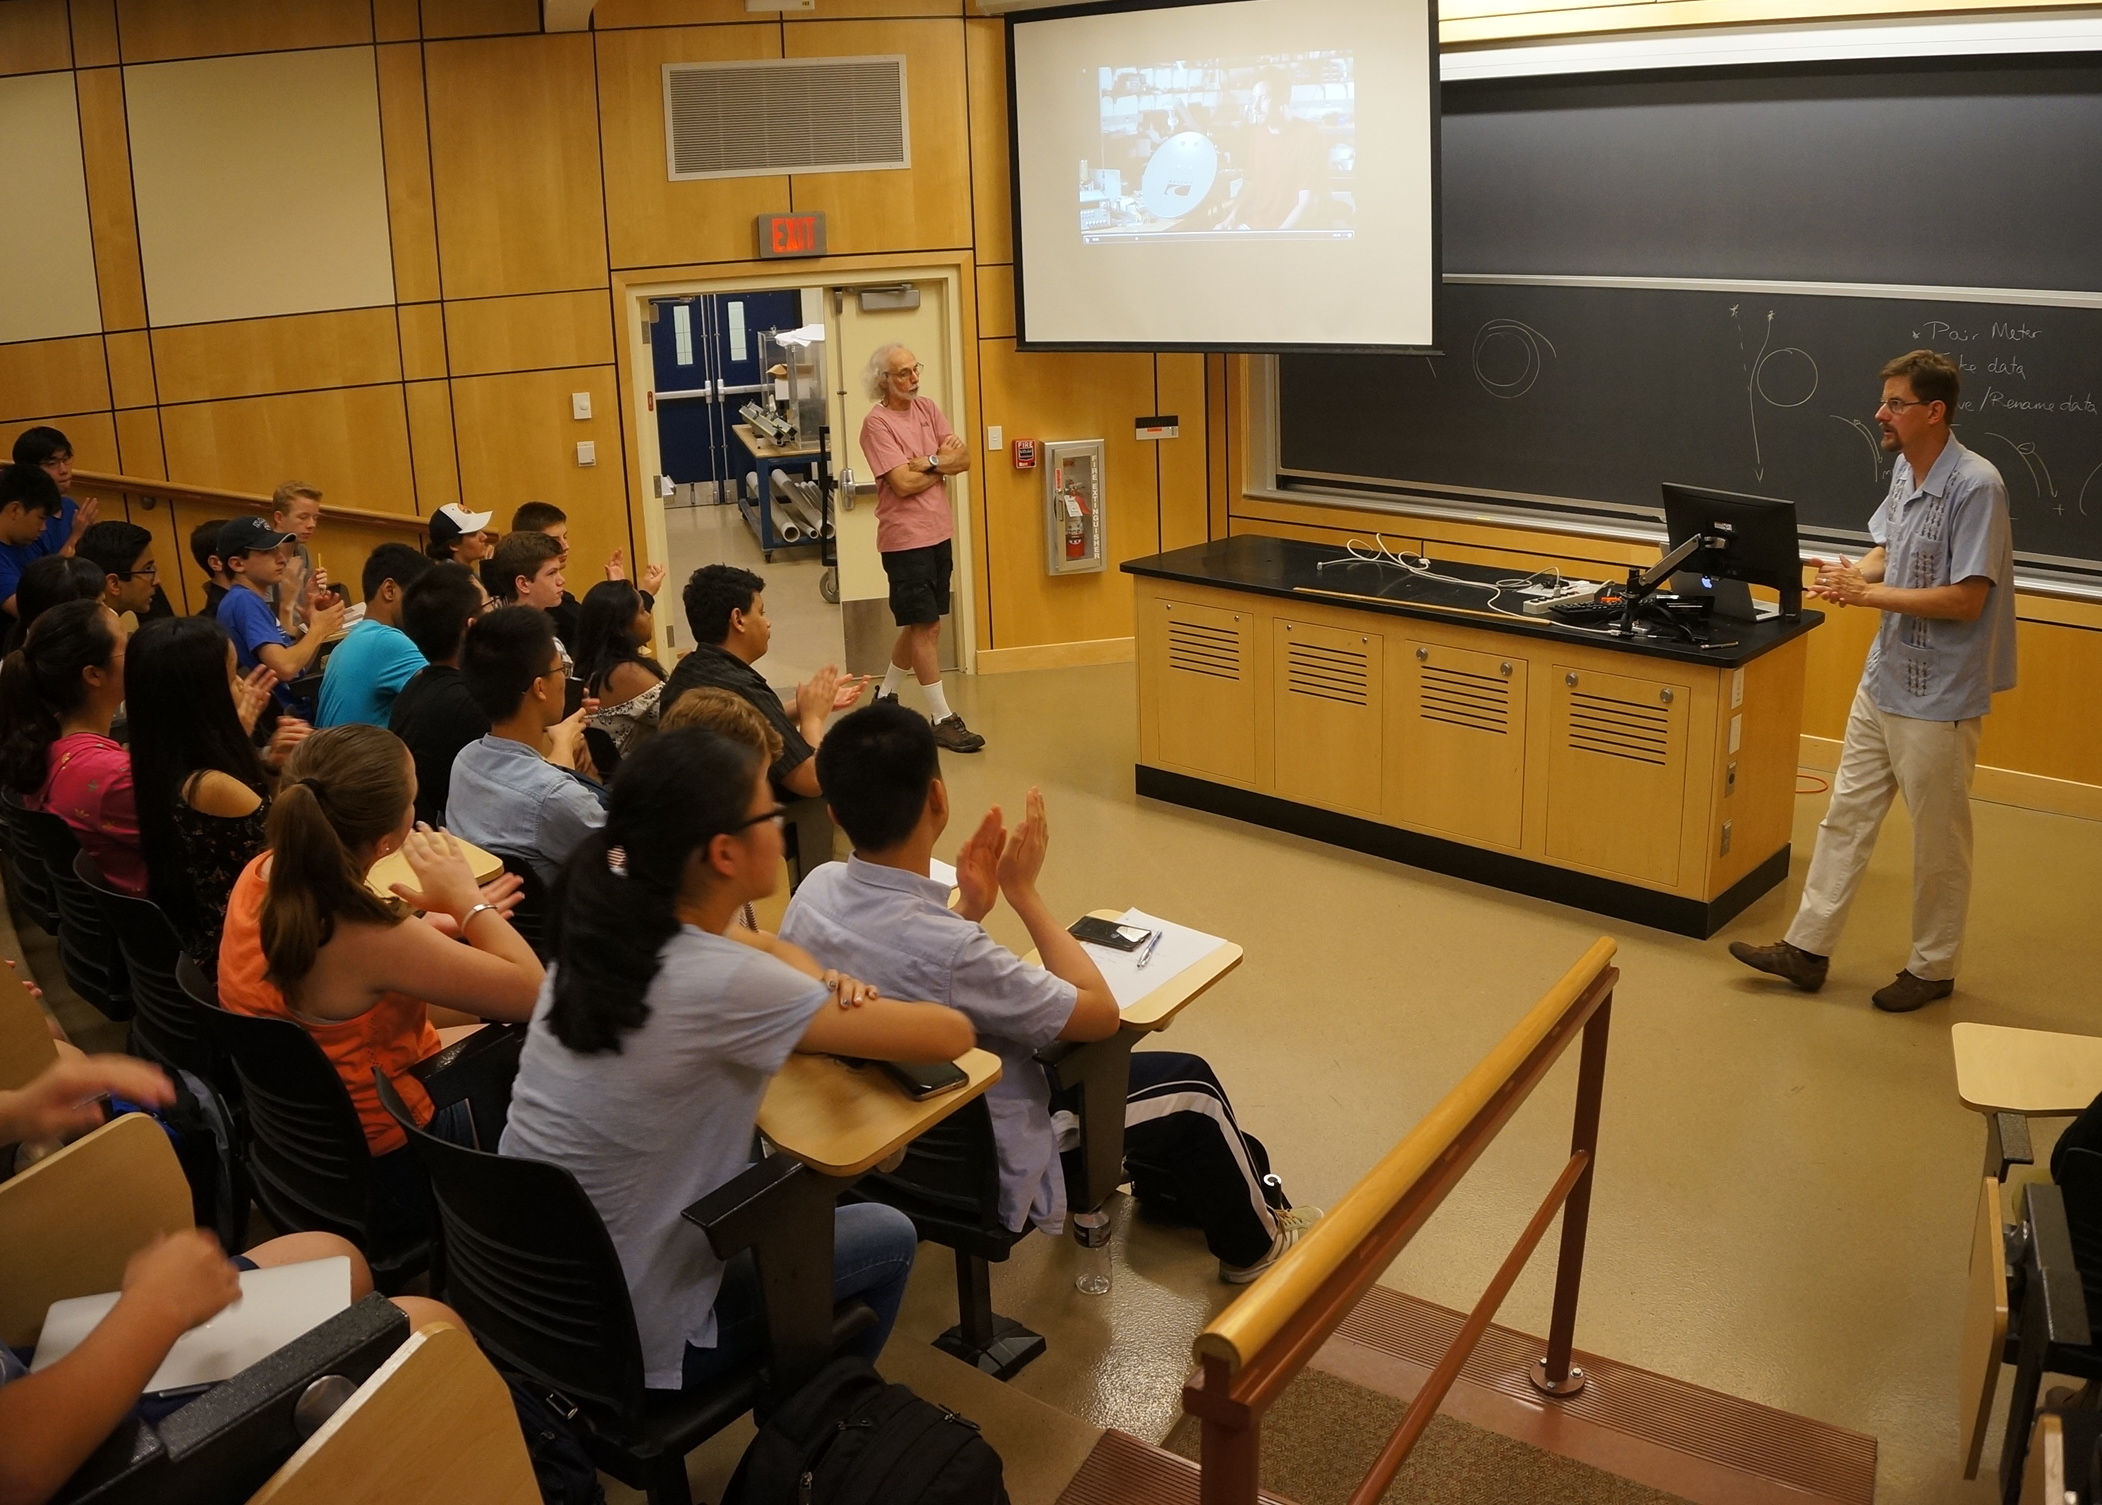
\includegraphics[width=6.5in]{EPRA_Lecture.jpg}
\vspace{5pt}
\caption{Prof.~Aguirre delivering a lecture to the high school students of the Experimental Physics Research Academy at Penn, Summer 2017.  
%The projected image is of the video describing his work at \url{https://penntoday.upenn.edu/spotlights/building-community-radio-telescope-west-philly}, but the video seems to have disappeared.
}
\label{fig:Devices}
\end{figure}

\begin{figure}[h]
\centering
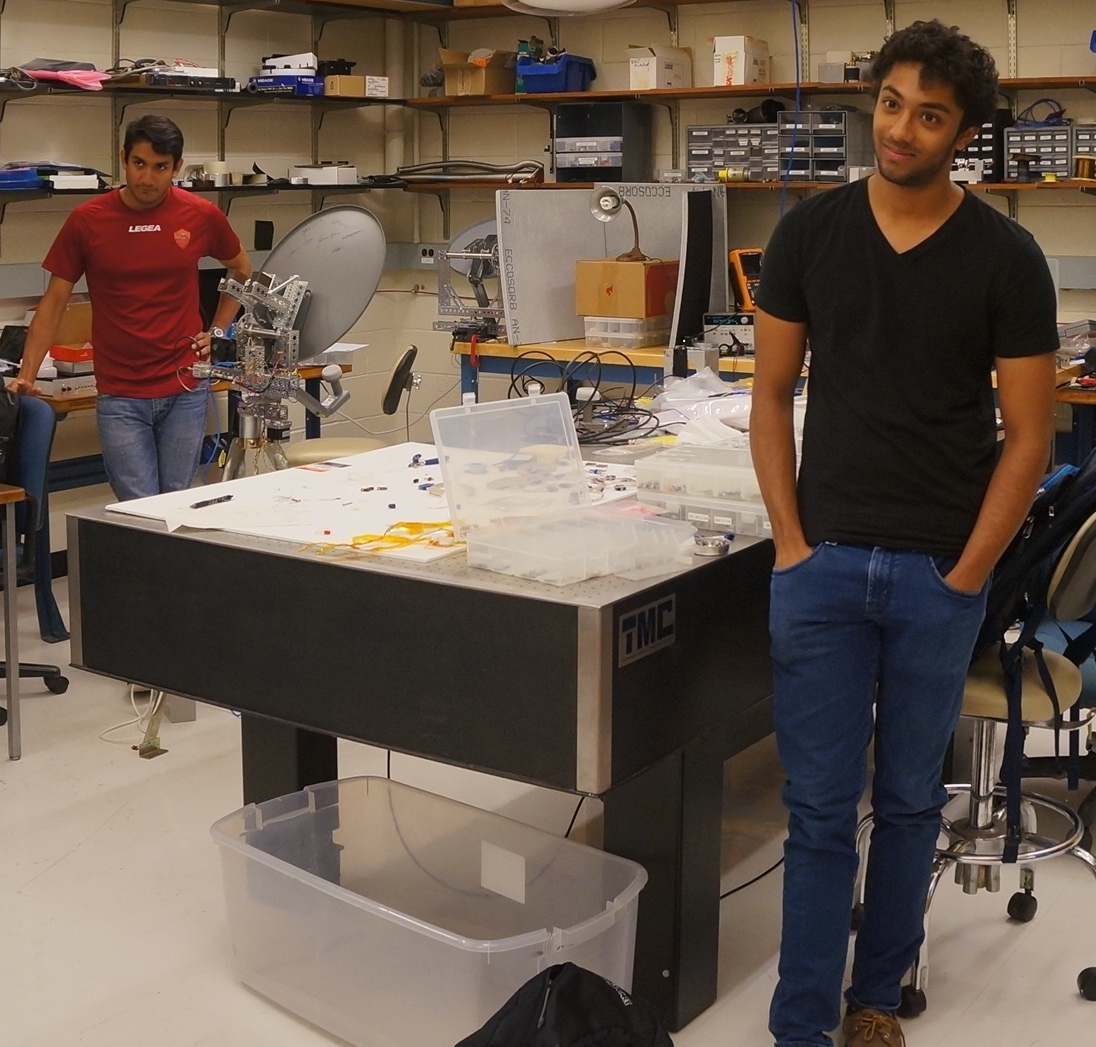
\includegraphics[width=6.5in]{DiazAndMenon.jpg}
\vspace{5pt}
\caption{Undergraduate research assistants Mauricio Diaz (left) and Viruj Menon (right) prepare to welcome the EPRA students.}
\label{fig:Devices}
\end{figure}

\begin{figure}[h]
\centering
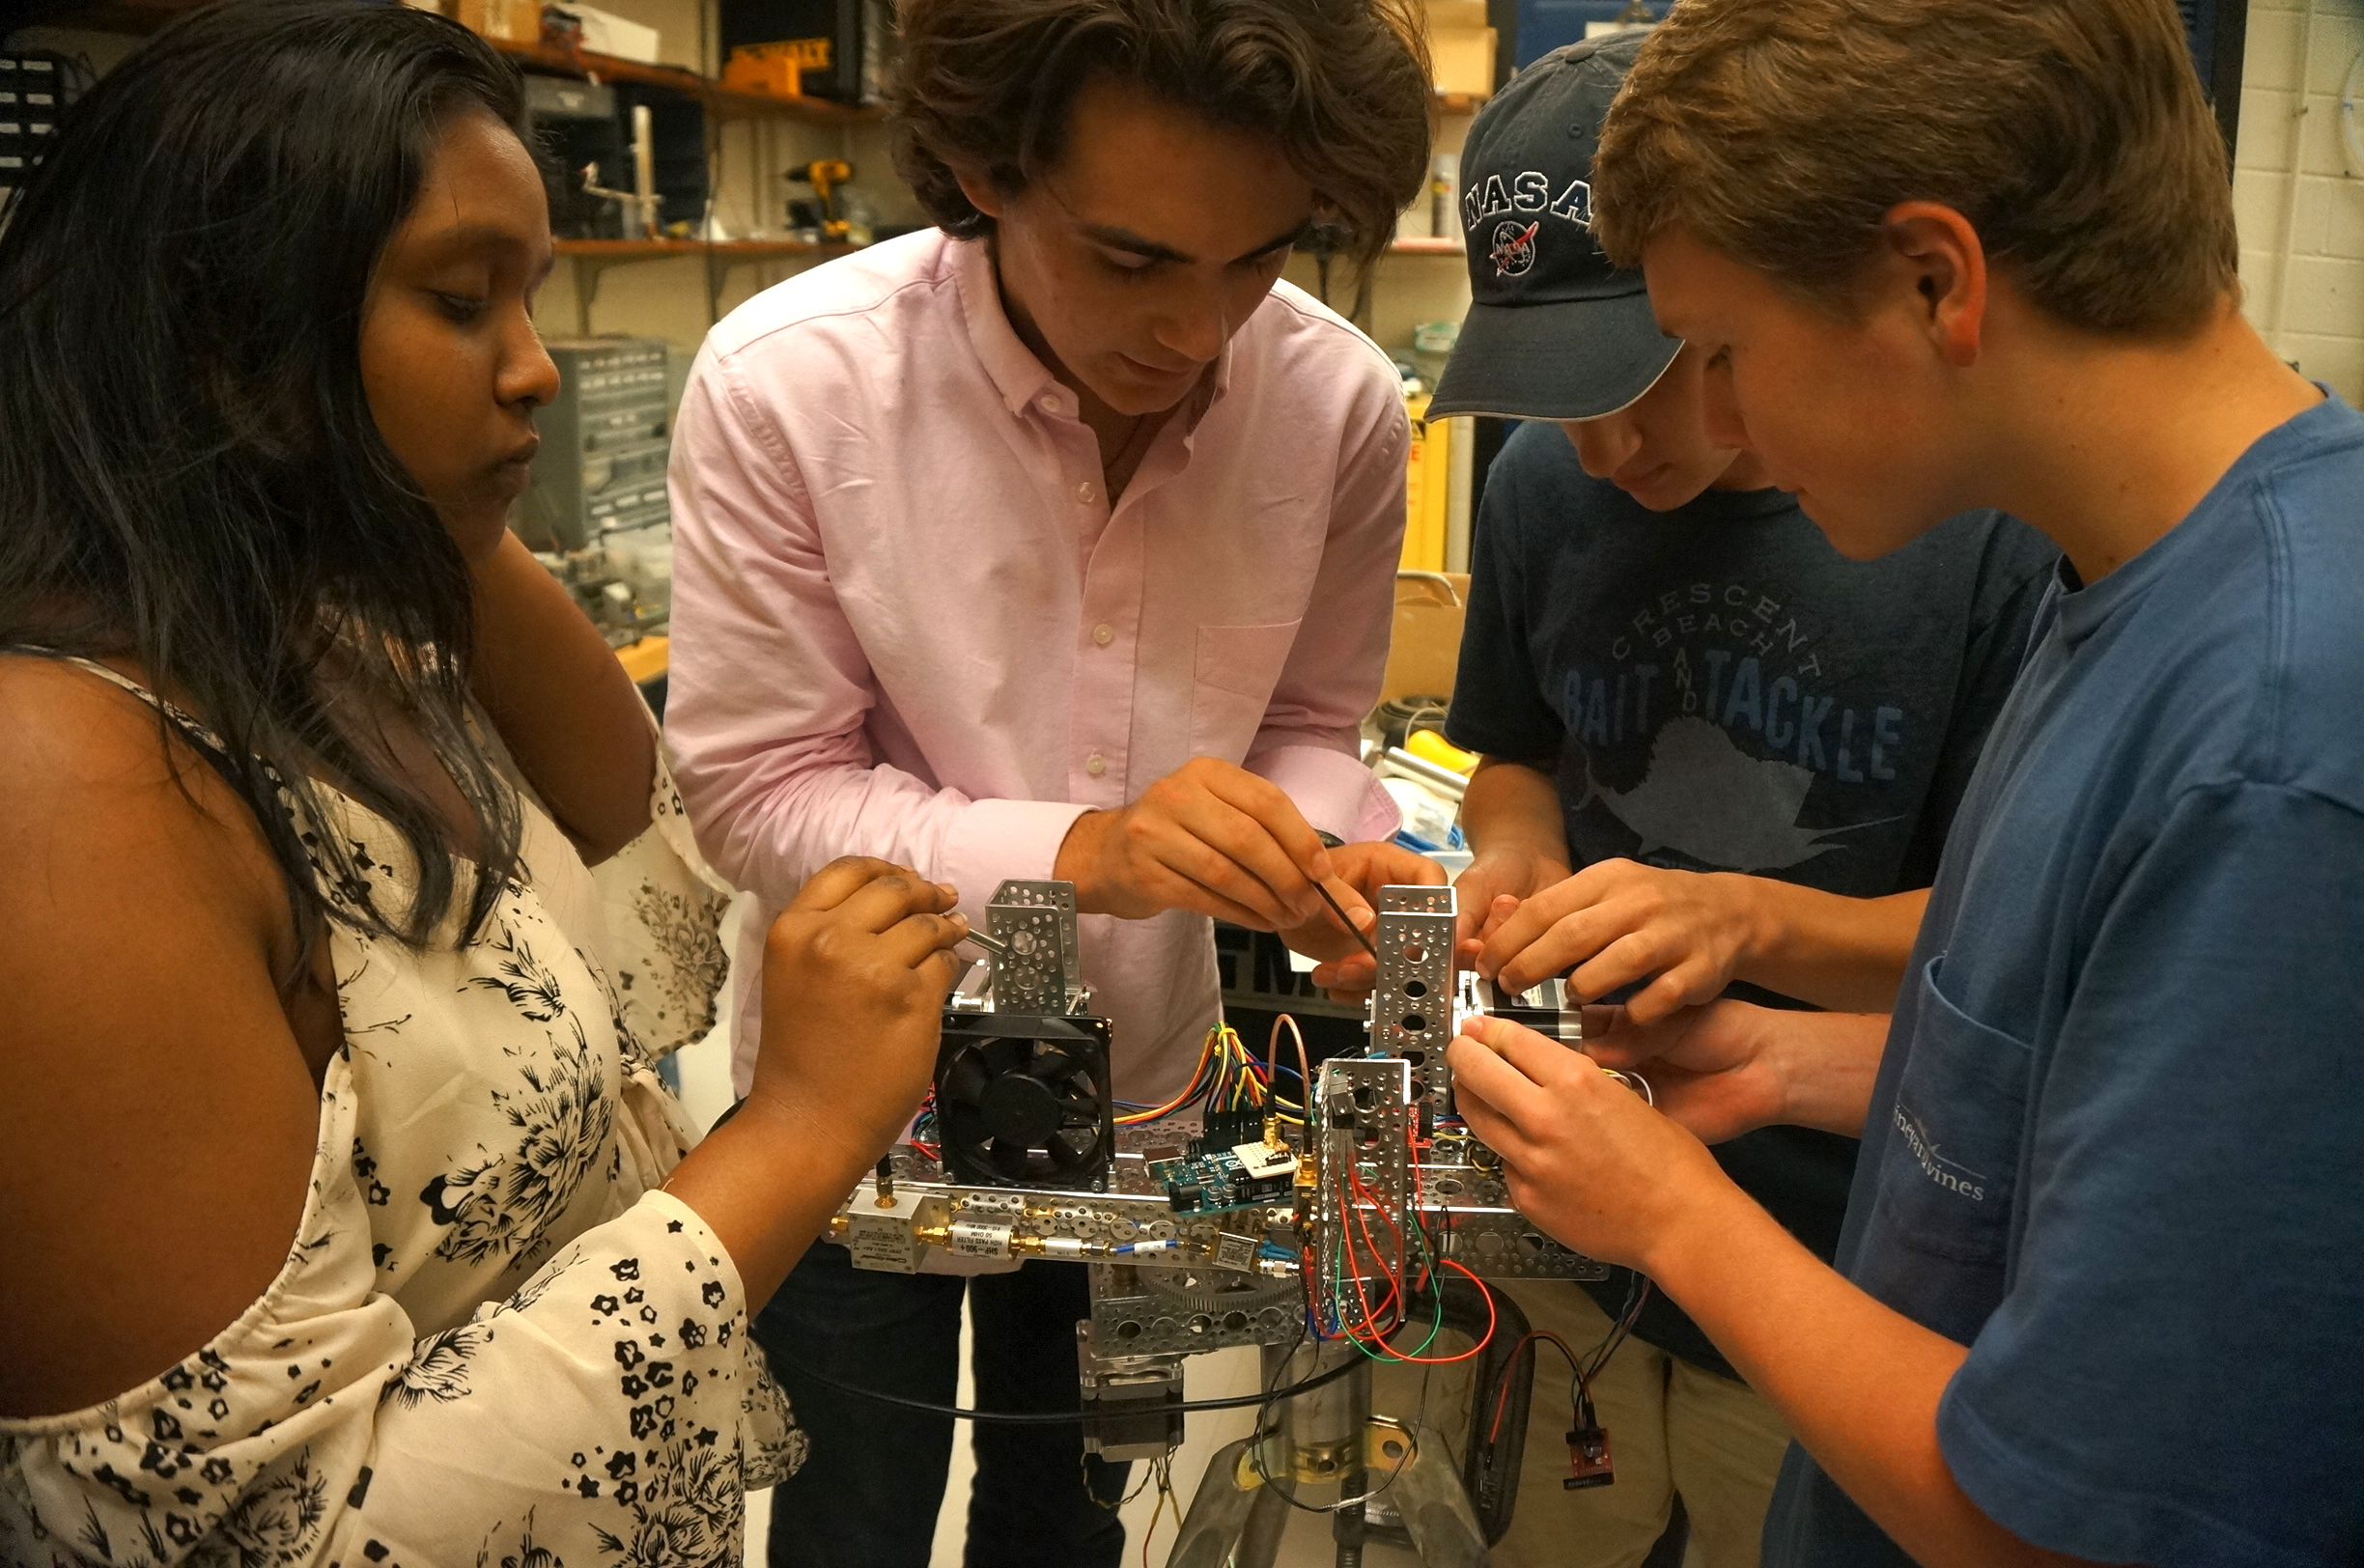
\includegraphics[width=6.5in]{EPRA_working.jpg}
\vspace{5pt}
\caption{EPRA students working on the MRT, summer 2017.}
\label{fig:Devices}
\end{figure}

\begin{figure}[h]
\centering
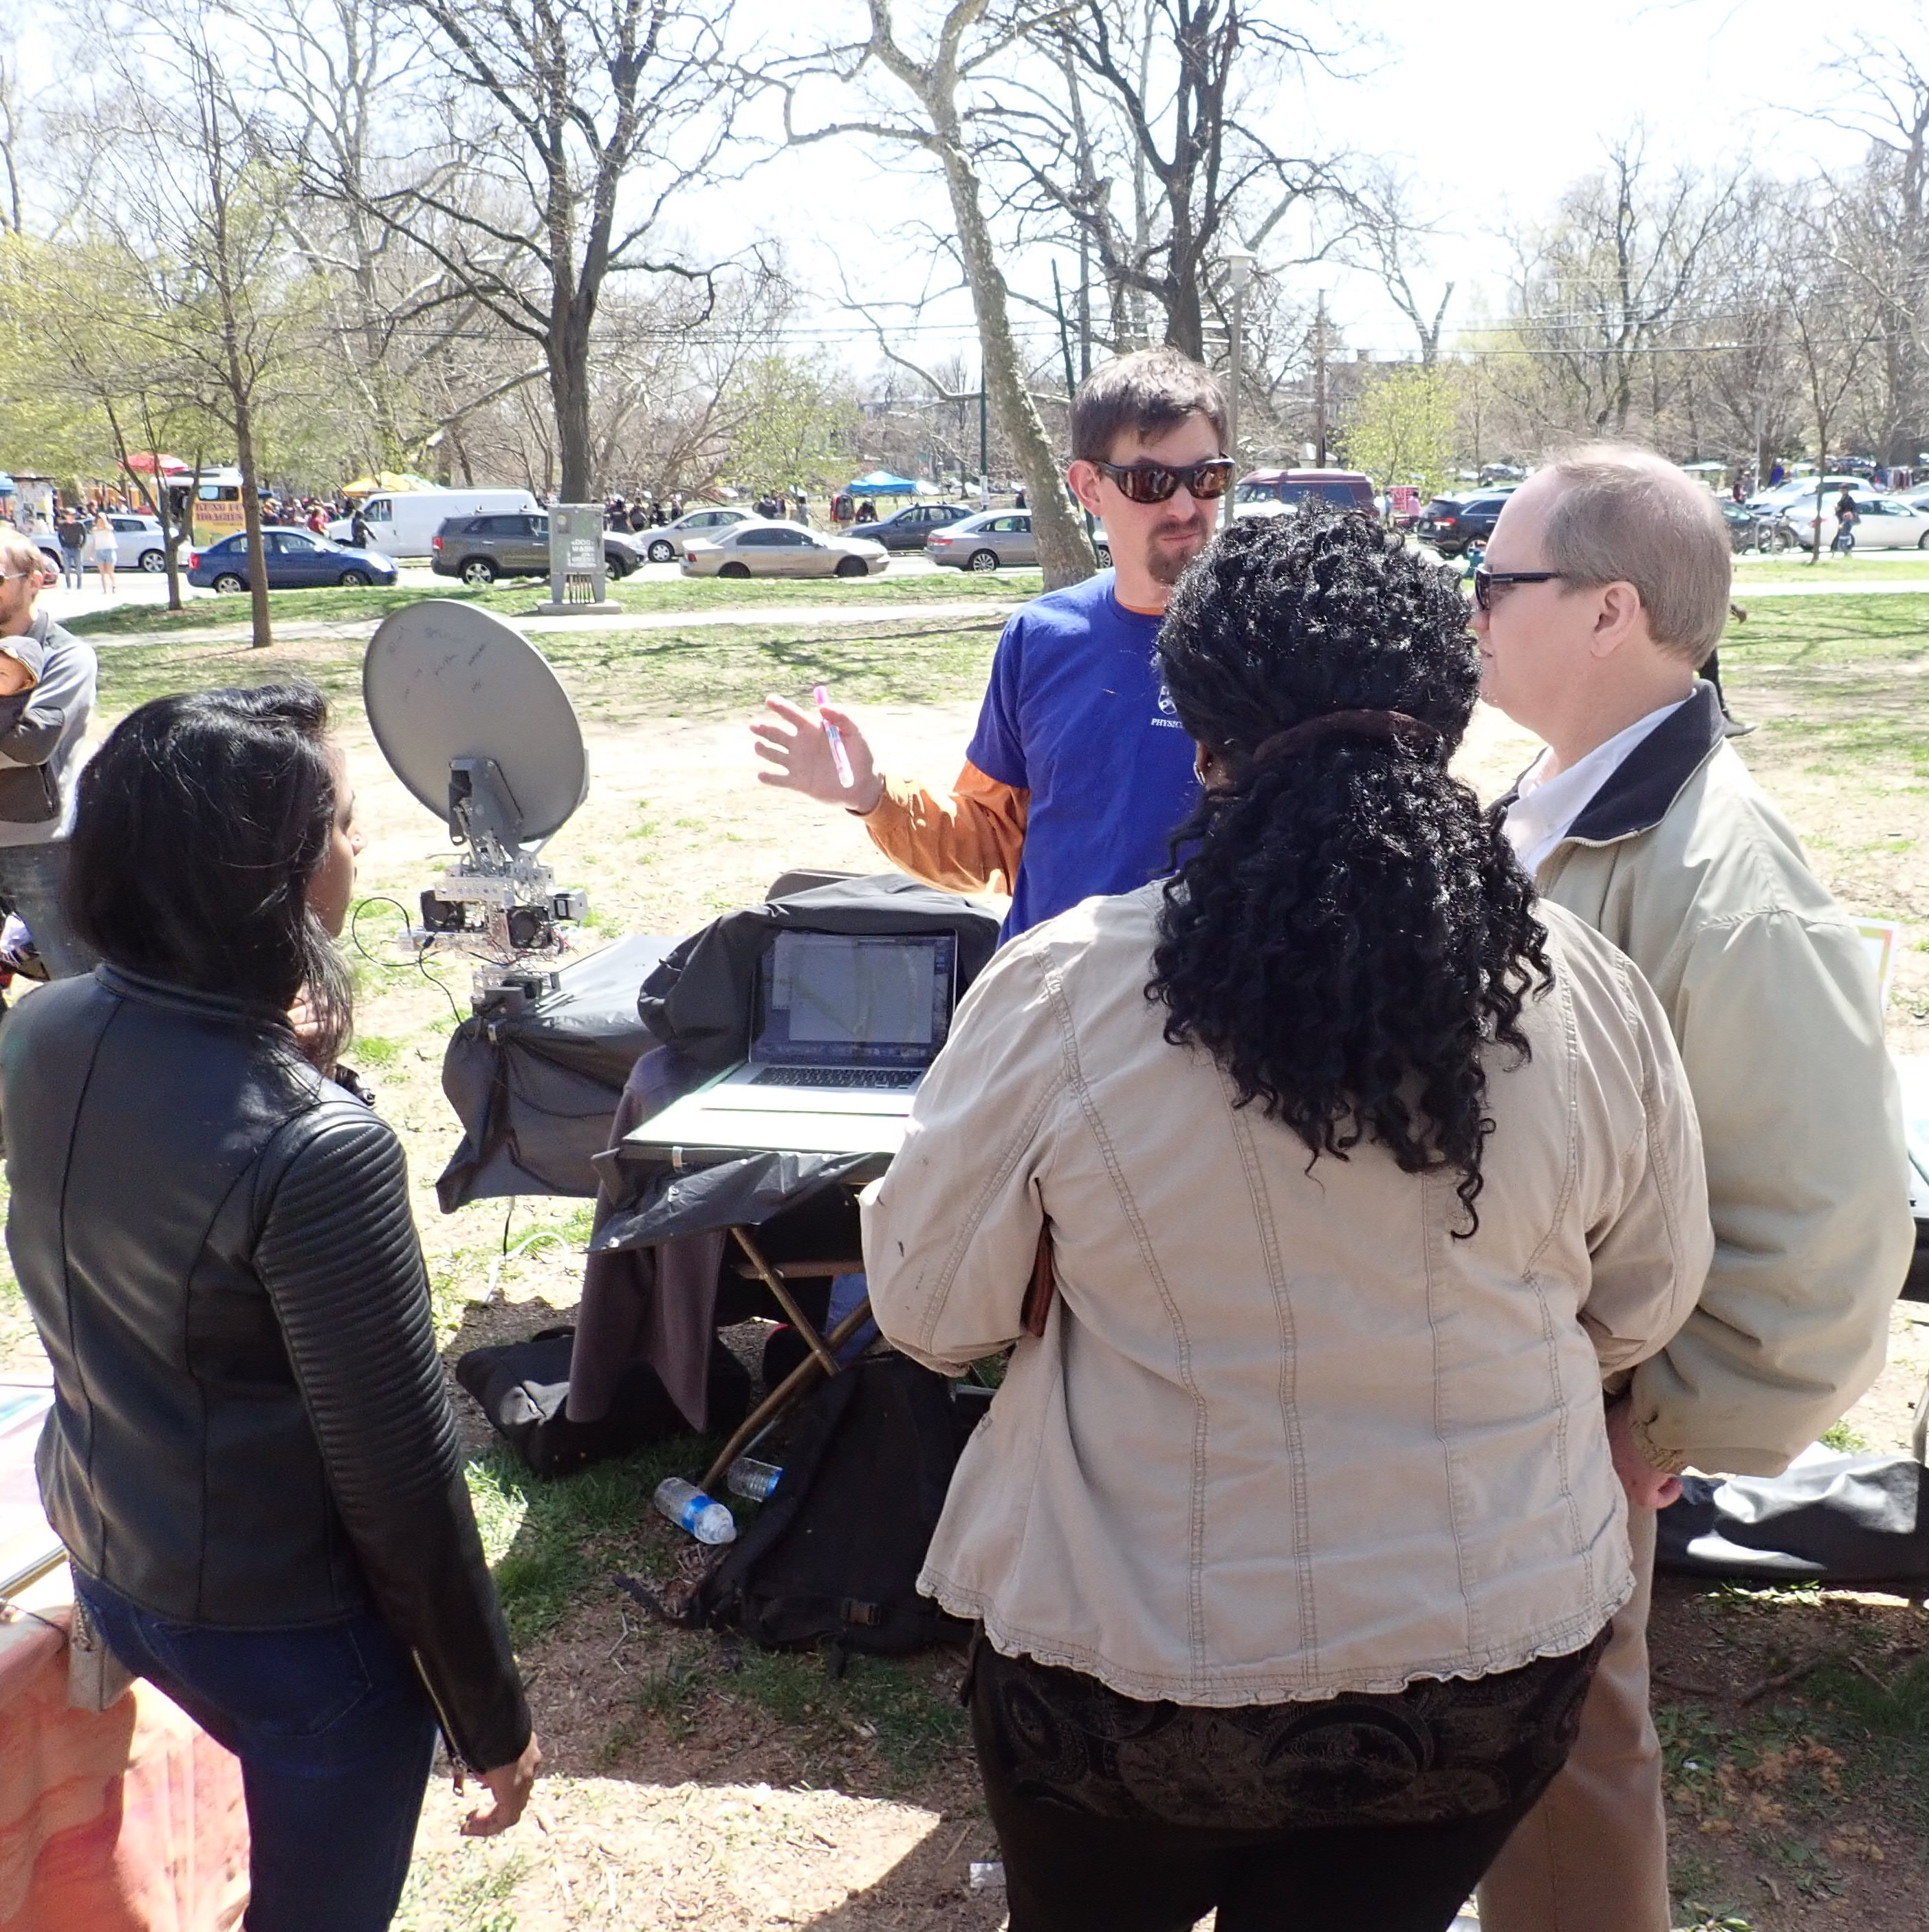
\includegraphics[width=6.5in]{ClarkPark.jpg}
\vspace{5pt}
\caption{Prof.~Aguirre with the MRT in Clark Park as part of the Philadelphia Science Festival, 21 April 2018.}
\label{fig:ClarkPark}
\end{figure}

\begin{figure}[h]
\centering
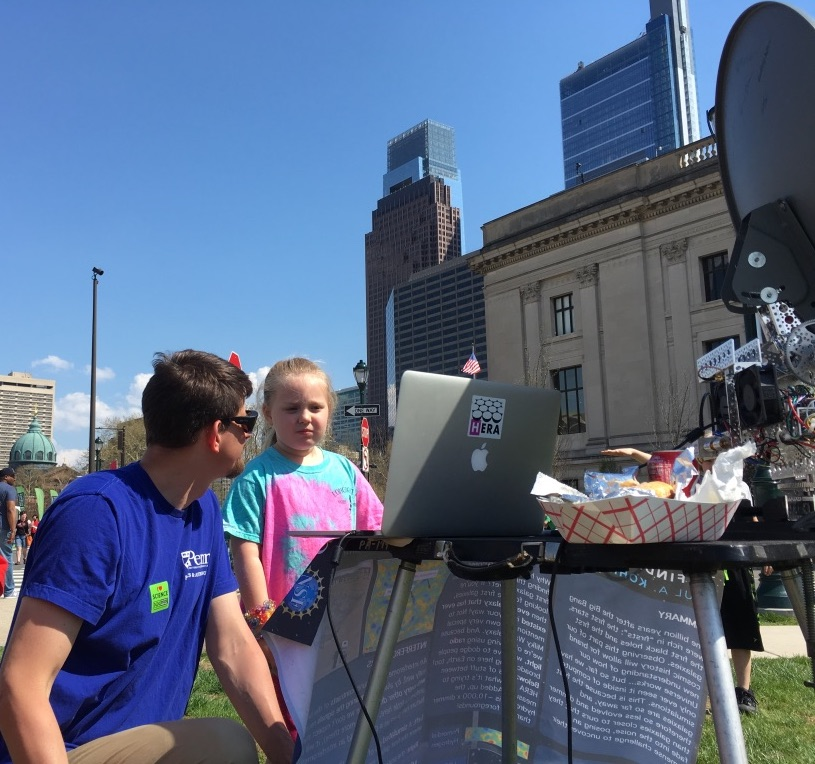
\includegraphics[width=6.5in]{PSFCarnival2.jpg}
\vspace{5pt}
\caption{Explaining the telescope to a young visitor to the Philadelphia Science Festival's Carnival, 28 April 2018.}
\label{fig:Devices}
\end{figure}

\end{document}


